\chapter{Specifikacija programske potpore}
		
	\section{Funkcionalni zahtjevi}
			
			\noindent \textbf{Dionici:}
			
			\begin{packed_enum}
				
				\item Klijenti
				\item Zaposlenici klinike:
					\begin{packed_enum}
						\item Doktori
						\item Treneri
					\end{packed_enum}
				\item Razvojni tim (grupa Flow)
				\item Naručitelj (asistent Hrvoje Nuić)
				\item Administratori aplikacije
				
			\end{packed_enum}
			
			\noindent \textbf{Aktori i njihovi funkcionalni zahtjevi:}
			
			
			\begin{packed_enum}
				\item  \underbar{Administrator (inicijator) može:}
				
				\begin{packed_enum}
					
					\item potvrditi ili odbiti željenu ulogu neregistriranom korisniku

					\item dodavati proizvode i vježbe u kategorije
					
					\item uređivati i brisati
					\begin{packed_enum}
						
						\item kategorije
						\item proizvode
						\item vježbe
						
					\end{packed_enum}
				\end{packed_enum}
			
				\item  \underbar{Doktor (inicijator) može:}
				
				\begin{packed_enum}
					
					\item odgovarati na recenzije svojih klijenata
					\item prekinuti suradnju s klijentom
					\item definirati dijetu svome klijentu
					\item pregledati statistiku svog klijenta
					\item dodavati proizvode i vježbe u kategorije	
					
				\end{packed_enum}
			
				\item  \underbar{Trener (inicijator) može:}
				
				\begin{packed_enum}
					
					\item odgovarati na recenzije svojih klijenata
					\item prekinuti suradnju s klijentom
					\item definirati treninge svome klijentu
					\item pregledati statistiku svog klijenta
					\item dodavati proizvode i vježbe u kategorije
					
				\end{packed_enum}
			
				\item  \underbar{Klijent (inicijator) može:}
				
				\begin{packed_enum}
					
					\item tražiti i pregledavati profile svih dostupnih doktora i trenera
					\item ostaviti recenziju svom doktoru ili treneru
					\item prekinuti suradnju sa svojim doktorom ili trenerom
					\item pregledati vlastitu statistiku
					\item provjeriti uklapa li se neki proizvod u dijetu skeniranjem bar koda ili ručnim unosom
					
				\end{packed_enum}
			
				\item  \underbar{Neregistrirani korisnik (inicijator) može:}
				
				\begin{packed_enum}
					
					\item registrirati se kao klijent
					\item poslati zahtjev za registraciju sa željenom ulogom
					
					\begin{packed_enum}
						
						\item trener
						\item doktor	
						
					\end{packed_enum}
					
				\end{packed_enum}
			
				\item  \underbar{Baza podataka (sudionik) može:}
				
				\begin{packed_enum}
					
					\item pohranjuje podatke o svim: 
					
					\begin{packed_enum}
						
						\item korisnicima i njihovim ovlastima
						\item recenzijama
						\item dijetama i proizvodima
						\item treninzima i vježbama
					
					\end{packed_enum}	
				
				\end{packed_enum}
			
			\end{packed_enum}
			
			\eject 
			
			
				
			\subsection{Obrasci uporabe}
					

					\noindent \underbar{\textbf{UC1 - Registracija klijenta}}
					\begin{packed_item}
	
						\item \textbf{Glavni sudionik:} Neregistrirani korisnik
						\item  \textbf{Cilj:} Stvoriti korisnički račun za pristup sustavu kao klijent
						\item  \textbf{Sudionici:} Baza podataka
						\item  \textbf{Preduvjet:} -
						\item  \textbf{Opis osnovnog tijeka:}
						
						\item[] \begin{packed_enum}
	
							\item Korisnik odabire opciju za registraciju klijenata
							\item Korisnik unosi potrebne podatke
							\item Korisnik potvrđuje podatke
							\item Sustav stvara novi korisnički račun i obavještava korisnika da je registracija uspješna
						\end{packed_enum}
						
						\item  \textbf{Opis mogućih odstupanja:}
						
						\item[] \begin{packed_item}
	
							\item[3.a] Unesesni podatci nisu ispravni
							\item[] \begin{packed_enum}
								
								\item Sustav obavještava korisnika o neuspjelom unosu i vraća ga na stranicu za registraciju
								\item Korisnik mijenja/dodaje potrebne podatke te završava unos ili odustaje od registracije
								
							\end{packed_enum}
							
						\end{packed_item}
					\end{packed_item}
				
					\noindent \underbar{\textbf{UC2 - Registracija zaposlenika}}
					\begin{packed_item}
						
						\item \textbf{Glavni sudionik:} Neregistrirani korisnik
						\item  \textbf{Cilj:} Stvoriti korisnički račun za pristup sustavu kao zaposlenik
						\item  \textbf{Sudionici:} Baza podataka
						\item  \textbf{Preduvjet:} -
						\item  \textbf{Opis osnovnog tijeka:}
						
						\item[] \begin{packed_enum}
							
							\item Korisnik odabire opciju za registraciju zaposlenika
							\item Korisnik unosi potrebne podatke
							\item Korisnik potvrđuje podatke
							\item Administrator potvrđuje zahtjev za registracijom
							\item Sustav stvara novi korisnički račun
						\end{packed_enum}
						
						\item  \textbf{Opis mogućih odstupanja:}
						
						\item[] \begin{packed_item}
							
							\item[3.a] Uneseni podatci nisu ispravni 
							\item[] \begin{packed_enum}
								
								\item Sustav obavještava korisnika o neuspjelom unosu i vraća ga na stranicu za registraciju
								\item Korisnik mijenja/dodaje potrebne podatke te završava unos ili odustaje od registracije
								
							\end{packed_enum}
						
							\item[4.a] Administrator odbija zahtjev
							\item [] \begin{packed_enum}
								
								\item Korisnik ne dobiva pristup sustavu
							
							\end{packed_enum}
						\end{packed_item}
					\end{packed_item}
				
					\noindent \underbar{\textbf{UC3 - Prijava u sustav}}
					\begin{packed_item}
						
						\item \textbf{Glavni sudionik:} Neprijavljeni korisnik
						\item  \textbf{Cilj:} Dobiti pristup korisničkom sučelju
						\item  \textbf{Sudionici:} Baza podataka
						\item  \textbf{Preduvjet:} Korisnik je registriran
						\item  \textbf{Opis osnovnog tijeka:}
						
						\item[] \begin{packed_enum}
							
							\item Korisnik unosi podatke potrebne za prijavu
							\item Korisnik potvrđuje unos
							\item Sustav prijavljuje korisnika i prikazuje korisničko sučelje
						\end{packed_enum}
						
						\item  \textbf{Opis mogućih odstupanja:}
						
						\item[] \begin{packed_item}
							
							\item[2.a] Uneseni podatci nisu ispravni
							\item[] \begin{packed_enum}
								
								\item Sustav obavještava korisnika o neuspjeloj prijavi i vraća ga na stranicu za prijavu
								
							\end{packed_enum}
						
							\item[3.a] Administrator nije još potvrdio korisnikov zahtjev za registraciju
							\item[] \begin{packed_enum}
								
								\item Sustav obavještava korisnika da njegov zahtjev još nije prihvaćen
								
							\end{packed_enum}
							
						\end{packed_item}
					\end{packed_item}
				
					\noindent \underbar{\textbf{UC4 - Potvrda zahtjeva neregistriranog korisnika}}
					\begin{packed_item}
						
						\item \textbf{Glavni sudionik:} Administrator
						\item  \textbf{Cilj:}  Potvrditi zahtjev neregistriranog korisnika
						\item  \textbf{Sudionici:} Baza podataka
						\item  \textbf{Preduvjet:} Korisnik je prijavljen
						\item  \textbf{Opis osnovnog tijeka:}
						
						\item[] \begin{packed_enum}
							
							\item Korisnik odabire prikaz zahtjeva za registraciju
							\item Korisnik potvrđuje željeni zahtjev
							\item Sustav stvara novi korisnički račun za osobu koja je poslala zahtjev
							
						\end{packed_enum}
						
						\item  \textbf{Opis mogućih odstupanja:}
						
						\item[] \begin{packed_item}
							
							\item[2.a] Zahtjev nije valjan
							\item[] \begin{packed_enum}
								
								\item Korisnik odbija zahtjev
								\item Sustav briše odbijeni zahtjev
								\item Sustav ponovo prikazuje zahtjeve za registracijom
								
							\end{packed_enum}
							
						\end{packed_item}
						
					\end{packed_item}
				
				
					\noindent \underbar{\textbf{UC5 - Slanje zahtjeva za suradnju}}
					\begin{packed_item}
						
						\item \textbf{Glavni sudionik:} Klijent
						\item  \textbf{Cilj:} Započeti suradnju sa željenim zaposlenikom
						\item  \textbf{Sudionici:} Baza podataka
						\item  \textbf{Preduvjet:} Korisnik je prijavljen
						\item  \textbf{Opis osnovnog tijeka:}
						
						\item[] \begin{packed_enum}
							
							\item Korisnik odabire pregled zaposlenika
							\item Korisnik odabire opciju za slanje zahtjeva željenom zaposleniku
							\item Zaposlenik kojem je slan zahtjev potvrđuje korisnika
							\item Korisnik i zaposlenik sada su u suradnji i sustav pohranjuje promjene u bazu podataka
							
						\end{packed_enum}
					
						\item	\textbf{Opis mogućih odstupanja:}
						
						\item[] \begin{packed_enum}
							
							\item[3.a] Zaposlenik odbija zahtjev
							\item[] \begin{packed_enum}
								
								\item Sustav obavještava korisnika da je njegov zahtjev odbijen
								
							\end{packed_enum}
						
						\end{packed_enum}
						
					\end{packed_item}
				
					\noindent \underbar{\textbf{UC6 - Potvrda zahtjeva za suradnju}}
					\begin{packed_item}
						
						\item \textbf{Glavni sudionik:} Doktor, trener
						\item  \textbf{Cilj:} Potvrditi zahtjev za suradnju koji je poslao klijent
						\item  \textbf{Sudionici:} Baza podataka
						\item  \textbf{Preduvjet:} Korisnik je prijavljen
						\item  \textbf{Opis osnovnog tijeka:}
						
						\item[] \begin{packed_enum}
							
							\item Korisnik odabire pregled zahtjeva za suradnju
							\item Korisnik potvrđuje željeni zahtjev
							\item Korisnik i klijent sada su u suradnji i sustav pohranjuje promjene u bazu podataka
							
						\end{packed_enum}
						
						\item  \textbf{Opis mogućih odstupanja:}
						
						\item[] \begin{packed_item}
							
							\item[2.a] Zahtjev nije valjan
							\item[] \begin{packed_enum}
								
								\item Korisnik odbija zahtjev
								\item Sustav javlja klijentu da je njegov zahtjev odbijen
								\item Sustav ponovno prikazuje pregled zahtjeva za suradnjom
								
							\end{packed_enum}
							
						\end{packed_item}	
						
					\end{packed_item}
				
					\noindent \underbar{\textbf{UC7 - Prekid suradnje}}
					\begin{packed_item}
						
						\item \textbf{Glavni sudionik:} Klijent, doktor, trener
						\item  \textbf{Cilj:} Prekinuti suradnju s osobom
						\item  \textbf{Sudionici:} Baza podataka
						\item  \textbf{Preduvjet:} Korisnik mora biti prijavljen i u suradnji s barem jednom osobom
						\item  \textbf{Opis osnovnog tijeka:}
						
						\item[] \begin{packed_enum}
							
							\item Korisnik odabire pregled svojih suradnika
							\item Korisnik odabire opciju za prekid suradnje s željenom osobom
							\item Korisnik i odabrana osoba više nisu u suradnji i sustav pohranjuje promjene u bazu podataka
							
						\end{packed_enum}
						
					\end{packed_item}
				
					\noindent \underbar{\textbf{UC8 - Ocjenjivanje zaposlenika}}
					\begin{packed_item}
						
						\item \textbf{Glavni sudionik:} Klijent
						\item  \textbf{Cilj:} Napisati recenziju zaposlenika s kojim je klijent u suradnji
						\item  \textbf{Sudionici:} Baza podataka
						\item  \textbf{Preduvjet:} Korisnik je prijavljen i u suradnji je s barem jednom osobom
						\item  \textbf{Opis osnovnog tijeka:}
						
						\item[] \begin{packed_enum}
							
							\item Korisnik odabire prikaz osoba s kojima je u suradnji
							\item Korisnik odabire kojeg zaposlenika želi ocijeniti
							\item Korisnik izabire ocjenu i piše komentar
							\item Korisnik potvrđuje unos
							\item Sustav pohranjuje recenziju u bazu podataka i ažurira prosječnu ocjenu zaposlenika
							
						\end{packed_enum}
					
						\item  \textbf{Opis mogućih odstupanja:}
						
						\item[] \begin{packed_item}
							
							\item[4.a] Nisu uneseni svi potrebni podatci
							\item[] \begin{packed_enum}
								
								\item Sustav obavještava korisnika da treba ispuniti sve potrebne podatke i vraća ga na stranicu za pisanje recenzije
								
							\end{packed_enum}
							
						\end{packed_item}
						
						
					\end{packed_item}
			
					\noindent \underbar{\textbf{UC9 - Odgovor na vlastitu recenziju}}
					\begin{packed_item}
						
						\item \textbf{Glavni sudionik:} Doktor, trener
						\item  \textbf{Cilj:} Odgovoriti na klijentovu recenziju
						\item  \textbf{Sudionici:} Baza podataka
						\item  \textbf{Preduvjet:} Korisnik je prijavljen i barem jedan klijent je napisao recenziju za njega
						\item  \textbf{Opis osnovnog tijeka:}
						
						\item[] \begin{packed_enum}
							
							\item Korisnik odabire pregled svojih recenzija
							\item Korisnik odabire opciju za odgovoriti na željenu recenziju
							\item Korisnik unosi potrebne podatke
							\item Korisnik potvrđuje unos
							\item Sustav pohranjuje odgovor u bazu podataka
							
						\end{packed_enum}
					
						\item  \textbf{Opis mogućih odstupanja:}
						
						\item[] \begin{packed_item}
							
							\item[4.a] Nisu uneseni svi potrebni podatci
							\item[] \begin{packed_enum}
								
								\item Sustav obavještava korisnika da treba ispuniti sve potrebne podatke i vraća ga na stranicu za odgovor na recenziju
								
							\end{packed_enum}
							
						\end{packed_item}
						
					\end{packed_item}
				
			
					\noindent \underbar{\textbf{UC10 - Definiranje dijete}}
					\begin{packed_item}
						
						\item \textbf{Glavni sudionik:} Doktor
						\item  \textbf{Cilj:} Definitrati dijetu svome klijentu
						\item  \textbf{Sudionici:} Baza podataka
						\item  \textbf{Preduvjet:} Korisnik je prijavljen i u suradnji je s barem jednim klijentom
						\item  \textbf{Opis osnovnog tijeka:}
						
						\item[] \begin{packed_enum}
							
							\item Korisnik odabire pregled svojih klijenata
							\item Korisnik odabire opciju za definiranje dijete željenom klijentu
							\item Korisnik unosi potrebne podatke
							\item Korisnik potvrđuje unos
							\item Sustav pohranjuje promjene u bazu podataka
							
						\end{packed_enum}
					
						\item  \textbf{Opis mogućih odstupanja:}
						
						\item[] \begin{packed_item}
							
							\item[4.a] Nisu uneseni svi potrebni podatci
							\item[] \begin{packed_enum}
								
								\item Sustav obavještava korisnika da treba ispuniti sve potrebne podatke i vraća ga na stranicu za definiranje dijete
								
							\end{packed_enum}
							
						\end{packed_item}
						
					\end{packed_item}
				
					\noindent \underbar{\textbf{UC11 - Definiranje treninga}}
					\begin{packed_item}
						
						\item \textbf{Glavni sudionik:} Trener
						\item  \textbf{Cilj:} Definirati trening svome klijentu
						\item  \textbf{Sudionici:} Baza podataka
						\item  \textbf{Preduvjet:} Korisnik je prijavljen i u suradnji s barem jednim klijentom
						\item  \textbf{Opis osnovnog tijeka:}
						
						\item[] \begin{packed_enum}
							
							\item Korisnik odabire prikaz svojih klijenata
							\item Korisnik odabire opciju za definiranje treninga željenom klijentu
							\item Korisnik unosi potrebne podatke
							\item Korisnik potvrđuje unos
							\item Sustav pohranjuje promjene u bazu podataka
							
						\end{packed_enum}
						
						\item  \textbf{Opis mogućih odstupanja:}
						
						\item[] \begin{packed_item}
							
							\item[4.a] Nisu uneseni svi potrebni podatci
							\item[] \begin{packed_enum}
								
								\item Sustav obavještava korisnika da treba ispuniti sve potrebne podatke i vraća ga na stranicu za definiranje treninga
								
							\end{packed_enum}
							
						\end{packed_item}
						
					\end{packed_item}
			
					\noindent \underbar{\textbf{UC12 - Pregled statistike klijenta}}
					\begin{packed_item}
						
						\item \textbf{Glavni sudionik:} Doktor, trener
						\item  \textbf{Cilj:} Pregledati statustiku klijenta po danu
						\item  \textbf{Sudionici:} Baza podataka
						\item  \textbf{Preduvjet:} Korisnik je prijavljen i u suradnji je s barem jednim klijentom
						\item  \textbf{Opis osnovnog tijeka:}
						
						\item[] \begin{packed_enum}
							
							\item Korisnik odabire pregled svojih klijenata
							\item Korisnik odabire opciju za pregled statistike željenog klijenta
							\item Korisnik odabire za koji dan se prikazuje statistika
							\item Sustav prikazuje statistiku klijenta za taj dan
							
						\end{packed_enum}
					
						\item  \textbf{Opis mogućih odstupanja:}
						
						\item[] \begin{packed_item}
							
							\item[4.a] Klijent nema upisanih podataka 
							\item[] \begin{packed_enum}
								
								\item Sustav obavještava da klijent nema upisanih podataka za taj dan i nudi opciju za povratak
								
							\end{packed_enum}
							
						\end{packed_item}	
						
					\end{packed_item}
			
					\noindent \underbar{\textbf{UC13 - Pregled svoje statistike}}
					\begin{packed_item}
						
						\item \textbf{Glavni sudionik:} Klijent
						\item  \textbf{Cilj:} Pregledati svoju statistiku po danu
						\item  \textbf{Sudionici:} Baza podataka
						\item  \textbf{Preduvjet:} Korisnik je prijavljen
						\item  \textbf{Opis osnovnog tijeka:}
						
						\item[] \begin{packed_enum}
							
							\item Korisnik odabire opciju za prikaz statistike
							\item Korisnik odabire za koji dan se prikazuje statistika
							\item Sustav prikazuje statistiku za taj dan
							
						\end{packed_enum}
					
						\item  \textbf{Opis mogućih odstupanja:}
						
						\item[] \begin{packed_item}
							
							\item[3.a] Klijent nema upisanih podataka 
							\item[] \begin{packed_enum}
								
								\item Sustav obavještava da nema upisanih podataka i nudi opciju za povratak
								
							\end{packed_enum}
							
						\end{packed_item}
						
					\end{packed_item}
			
					\noindent \underbar{\textbf{UC14 - Dodavanje proizvoda u kategoriju}}
					\begin{packed_item}
						
						\item \textbf{Glavni sudionik:} Doktor, trener, administrator
						\item  \textbf{Cilj:} Dodati proizvod u željenu kategoriju
						\item  \textbf{Sudionici:} Baza podataka
						\item  \textbf{Preduvjet:} Korisnik je prijavljen
						\item  \textbf{Opis osnovnog tijeka:}
						
						\item[] \begin{packed_enum}
							
							\item Korisnik odabire prikaz kategorija proizvoda
							\item Korisnik odabire željenu kategoriju
							\item Korisnik dodaje željene proizvode u kategoriju
							\item Sustav pohranjuje promjene bazu podataka
							
						\end{packed_enum}
					
					\end{packed_item}
			
					\noindent \underbar{\textbf{UC15 - Dodavanje vježbe u kategoriju}}
					\begin{packed_item}
						
						\item \textbf{Glavni sudionik:} Doktor, trener, administrator
						\item  \textbf{Cilj:} Dodati vježbu u željenu kategoriju
						\item  \textbf{Sudionici:} Baza podataka
						\item  \textbf{Preduvjet:} Korisnik je prijavljen
						\item  \textbf{Opis osnovnog tijeka:}
						
						\item[] \begin{packed_enum}
							
							\item Korisnik odabire prikaz kategorija vježbi
							\item Korisnik odabire željenu kategoriju
							\item Korisnik dodaje željene vježbe u kategoriju
							\item Sustav pohranjuje promjene u bazu podataka
							
						\end{packed_enum}
						
					\end{packed_item}
			
					\noindent \underbar{\textbf{UC16 - Stvaranje kategorije}}
					\begin{packed_item}
						
						\item \textbf{Glavni sudionik:} Administrator
						\item  \textbf{Cilj:} Stvoriti novu kategoriju
						\item  \textbf{Sudionici:} Baza podataka
						\item  \textbf{Preduvjet:} Korisnik je prijavljen
						\item  \textbf{Opis osnovnog tijeka:}
						
						\item[] \begin{packed_enum}
							
							\item Korisnik odabire prikaz kategorija
							\item Korisnik odabire opciju za kreiranje nove kategorije
							\item Korisnik unosi potrebne podatke o kategoriji i njen sadržaj
							\item Korisnik potvrđuje unos
							\item Sustav pohranjuje novu kategoriju u bazu podataka
							
						\end{packed_enum}
						
						\item  \textbf{Opis mogućih odstupanja:}
						
						\item[] \begin{packed_item}
							
							\item[4.a] Nisu uneseni svi potrebni podatci
							\item[] \begin{packed_enum}
								
								\item Sustav obavještava korisnika da treba unijeti sve potrebne podatke i vraća ga na stranicu za stvaranje kategorije
								
							\end{packed_enum}
							
						\end{packed_item}
						
					\end{packed_item}
			
					\noindent \underbar{\textbf{UC17 - Uređivanje kategorija}}
					\begin{packed_item}
						
						\item \textbf{Glavni sudionik:} Administrator
						\item  \textbf{Cilj:} Izmijenti sadržaj kategorije i podatke o kategoriji
						\item  \textbf{Sudionici:} Baza podataka
						\item  \textbf{Preduvjet:} Korisnik je prijavljen i postoji barem jedna kategorija
						\item  \textbf{Opis osnovnog tijeka:}
						
						\item[] \begin{packed_enum}
							
							\item Korisnik odabire prikaz kategorija
							\item Korisnik odabire kategoriju koju želi izmijeniti
							\item Korisnik mijenja podatke o kategoriji i njen sadržaj
							\item Korisnik potvrđuje izmjenu
							\item Promjene se pohranjuju u bazu podataka
							
						\end{packed_enum}
						
						\item  \textbf{Opis mogućih odstupanja:}
						
						\item[] \begin{packed_item}
							
							\item[4.a] Izmijenjeni podatci nisu ispravni 
							\item[] \begin{packed_enum}
								
								\item Sustav obavještava korisnika da mora unijeti ispravne podatke i vraća ga na stranicu za uređivanje kategorije
								
							\end{packed_enum}
							
						\end{packed_item}
						
					\end{packed_item}
				
				
					\noindent \underbar{\textbf{UC18 - Brisanje kategorije}}
					\begin{packed_item}
						
						\item \textbf{Glavni sudionik:} Administrator
						\item  \textbf{Cilj:} Obrisati kategoriju
						\item  \textbf{Sudionici:} Baza podataka
						\item  \textbf{Preduvjet:} Korisnik je prijavljen i postoji barem jedna kategorija
						\item  \textbf{Opis osnovnog tijeka:}
						
						\item[] \begin{packed_enum}
							
							\item Korisnik odabire prikaz kategorija
							\item Korisnik odabire opciju za brisanje željene kategorije
							\item Sustav briše kategoriju i pohranjuje promjene u bazu podataka
							
						\end{packed_enum}
						
					\end{packed_item}
				
					\noindent \underbar{\textbf{UC19 - Dodavanje proizvoda}}
					\begin{packed_item}
						
						\item \textbf{Glavni sudionik:} Administrator
						\item  \textbf{Cilj:} Dodati novi proizvod u sustav
						\item  \textbf{Sudionici:} Baza podataka
						\item  \textbf{Preduvjet:} Korisnik je prijavljen
						\item  \textbf{Opis osnovnog tijeka:}
						
						\item[] \begin{packed_enum}
							
							\item Korisnik odabire prikaz proizvoda
							\item Korisnik odabire opciju za dodavanje novog proizvoda
							\item Korisnik unosi sve potrebne podatke
							\item Korisnik potvrđuje unos
							\item Sustav dodaje proizvod i pohranjuje ga u bazu podataka
							
						\end{packed_enum}
						
						\item  \textbf{Opis mogućih odstupanja:}
						
						\item[] \begin{packed_item}
							
							\item[4.a] Nisu uneseni svi potrebni podatci
							\item[] \begin{packed_enum}
								
								\item Sustav obavještava korisnika da treba unijeti sve potrebne podatke i vraća ga na stranicu za dodavanje proizvoda
								
							\end{packed_enum}
							
						\end{packed_item}	
							
					\end{packed_item}
				
					\noindent \underbar{\textbf{UC20 - Uređivanje proizvoda}}
					\begin{packed_item}
						
						\item \textbf{Glavni sudionik:} Administrator
						\item  \textbf{Cilj:} Izmijeniti podatke o željenom proizvodu
						\item  \textbf{Sudionici:} Baza podataka
						\item  \textbf{Preduvjet:} Korisnik je prijavljen i dodan je barem jedan proizvod
						\item  \textbf{Opis osnovnog tijeka:}
						
						\item[] \begin{packed_enum}
							
							\item Korisnik odabire prikaz proizvoda
							\item Korisnik odabire opciju za uređivanje željenog proizvoda
							\item Korisnik mijenja podatke o proizvodu
							\item Korisnik potvrđuje izmjenu
							\item Sustav pohranjuje promjenu u bazu podataka
							
						\end{packed_enum}
						
						\item  \textbf{Opis mogućih odstupanja:}
						
						\item[] \begin{packed_item}
							
							\item[4.a] Izmijenjeni podatci nisu ispravni 
							\item[] \begin{packed_enum}
								
								\item Sustav obavještava korisnika da mora unijeti ispravne podatke i vraća ga na stranicu za uređivanje proizvoda
								
							\end{packed_enum}
							
						\end{packed_item}	
						
					\end{packed_item}
				
					\noindent \underbar{\textbf{UC21 - Brisanje proizvoda}}
					\begin{packed_item}
						
						\item \textbf{Glavni sudionik:} Administrator
						\item  \textbf{Cilj:} Obrisati proizvod
						\item  \textbf{Sudionici:} Baza podataka
						\item  \textbf{Preduvjet:} Korisnik je prijavljen i dodan je barem jedan proizvod
						\item  \textbf{Opis osnovnog tijeka:}
						
						\item[] \begin{packed_enum}
							
							\item Korisnik odabire prikaz proizvoda
							\item Korisnik odabire opciju za brisanje željenog proizvoda
							\item Sustav briše proizvod i pohranjuje promjene u bazu podataka
							
						\end{packed_enum}
							
						
					\end{packed_item}
				
					\noindent \underbar{\textbf{UC22 - Dodavanje vježbe}}
					\begin{packed_item}
						
						\item \textbf{Glavni sudionik:} Administrator
						\item  \textbf{Cilj:} Dodati novu vježbu u sustav
						\item  \textbf{Sudionici:} Baza podataka
						\item  \textbf{Preduvjet:} Korisnik je prijavljen
						\item  \textbf{Opis osnovnog tijeka:}
						
						\item[] \begin{packed_enum}
							
							\item Korisnik odabire prikaz vježbi
							\item Korisnik odabire opciju za dodavanje vježbe
							\item Korisnik unosi sve potrebne podatke
							\item Korisnik potvrđuje unos
							\item Sustav stvara novu vježbu i pohranjuje izmijene u bazu podataka
							
						\end{packed_enum}
						
						\item  \textbf{Opis mogućih odstupanja:}
						
						\item[] \begin{packed_item}
							
							\item[4.a] Nisu uneseni svi potrebni podatci
							\item[] \begin{packed_enum}
								
								\item Sustav obavještava korisnika da treba unijeti sve potrebne podatke i vraća ga na stranicu za dodavanje vježbe
								
							\end{packed_enum}
							
						\end{packed_item}	
						
					\end{packed_item}
					
					\noindent \underbar{\textbf{UC23 - Uređivanje vježbe}}
					\begin{packed_item}
						
						\item \textbf{Glavni sudionik:} Administrator
						\item  \textbf{Cilj:} Izmijeniti podatke o željenoj vježbi
						\item  \textbf{Sudionici:} Baza podataka
						\item  \textbf{Preduvjet:} Korisnik je prijavljen i dodana je barem jedna vježba
						\item  \textbf{Opis osnovnog tijeka:}
						
						\item[] \begin{packed_enum}
							
							\item Korisnik odabire prikaz vježbi
							\item Korisnik odabire opciju za uređivanje željenog proizvoda
							\item Korisnik mijenja podatke o vježbi
							\item Korisnik potvrđuje izmjenu
							\item Sustav pohranjuje promjenu u bazu podataka
							
						\end{packed_enum}
						
						\item  \textbf{Opis mogućih odstupanja:}
						
						\item[] \begin{packed_item}
							
							\item[4.a] Izmijenjeni podatci nisu ispravni 
							\item[] \begin{packed_enum}
								
								\item Sustav obavještava korisnika da mora unijeti ispravne podatke i vraća ga na stranicu za uređivanje vježbe
								
							\end{packed_enum}
							
						\end{packed_item}	
						
					\end{packed_item}
					
					\noindent \underbar{\textbf{UC24 - Brisanje vježbe}}
					\begin{packed_item}
						
						\item \textbf{Glavni sudionik:} Administrator
						\item  \textbf{Cilj:} Obrisati vježbu
						\item  \textbf{Sudionici:} Baza podataka
						\item  \textbf{Preduvjet:} Korisnik je prijavljen i dodana je barem jedna vježba
						\item  \textbf{Opis osnovnog tijeka:}
						
						\item[] \begin{packed_enum}
							
							\item Korisnik odabire prikaz vježbi
							\item Korisnik odabire opciju za brisanje željene vježbe
							\item Sustav briše vježbu i promijene se pohranjuju u bazu podataka
							
						\end{packed_enum}
						
						
					\end{packed_item}
				
					\noindent \underbar{\textbf{UC25 - Provjera proizvoda skeniranjem}}
					\begin{packed_item}
						
						\item \textbf{Glavni sudionik:} Klijent
						\item  \textbf{Cilj:} Skenirati proizvod i odrediti uklapa li se u njegovu dijetu
						\item  \textbf{Sudionici:} Baza podataka
						\item  \textbf{Preduvjet:} Korisnik je prijavljen i pripisana mu je dijeta
						\item  \textbf{Opis osnovnog tijeka:}
						
						\item[] \begin{packed_enum}
							
							\item Korisnik odabire opciju za provjeru proizvoda
							\item Korisnik odabire skeniranje bar koda kao način provjere
							\item Korisnik fotografira bar kod proizvoda
							\item Sustav javlja korisniku uklapa li se proizvod u dijetu za taj dan
							
						\end{packed_enum}
						
						\item  \textbf{Opis mogućih odstupanja:}
						
						\item[] \begin{packed_item}
							
							\item[2.a] Bar kod nije prepoznat u slici
							\item[] \begin{packed_enum}
								
								\item Sustav javlja da je potrebno jasnije skenirati bar kod
								\item Korisnik ponovo skenira proizvod
								
							\end{packed_enum}
						
							\item[2.b] Sustav ne prepoznaje proizvod
							\item[] \begin{packed_enum}
								
								\item Sustav javlja da nema podatke o traženom proizvodu
								\item Sustav vraća korisnika na početno sučelje
								
							\end{packed_enum}
							
						\end{packed_item}
						
					\end{packed_item}
				
					\noindent \underbar{\textbf{UC26 - Provjera proizvoda ručnim unosom}}
					\begin{packed_item}
						
						\item \textbf{Glavni sudionik:} Klijent
						\item  \textbf{Cilj:} Unijeti masu proizvoda i odrediti uklapa li se u njegovu dijetu
						\item  \textbf{Sudionici:} Baza podataka
						\item  \textbf{Preduvjet:} Korisnik je prijavljen i pripisana mu je dijeta
						\item  \textbf{Opis osnovnog tijeka:}
						
						\item[] \begin{packed_enum}
							
							\item Korisnik odabire opciju provjere proizvoda
							\item Korisnik odabire ručni unos kao način provjere
							\item Korisnik odabire željeni proizvod i unosi količinu(masu) koju želi konzumirati
							\item Sustav javlja korisniku uklapa li se proizvod u dijetu za taj dan
							
						\end{packed_enum}
						
						
					\end{packed_item}
				
					
					
				\subsubsection{Dijagrami obrazaca uporabe}
					
					\begin{figure}[H]
						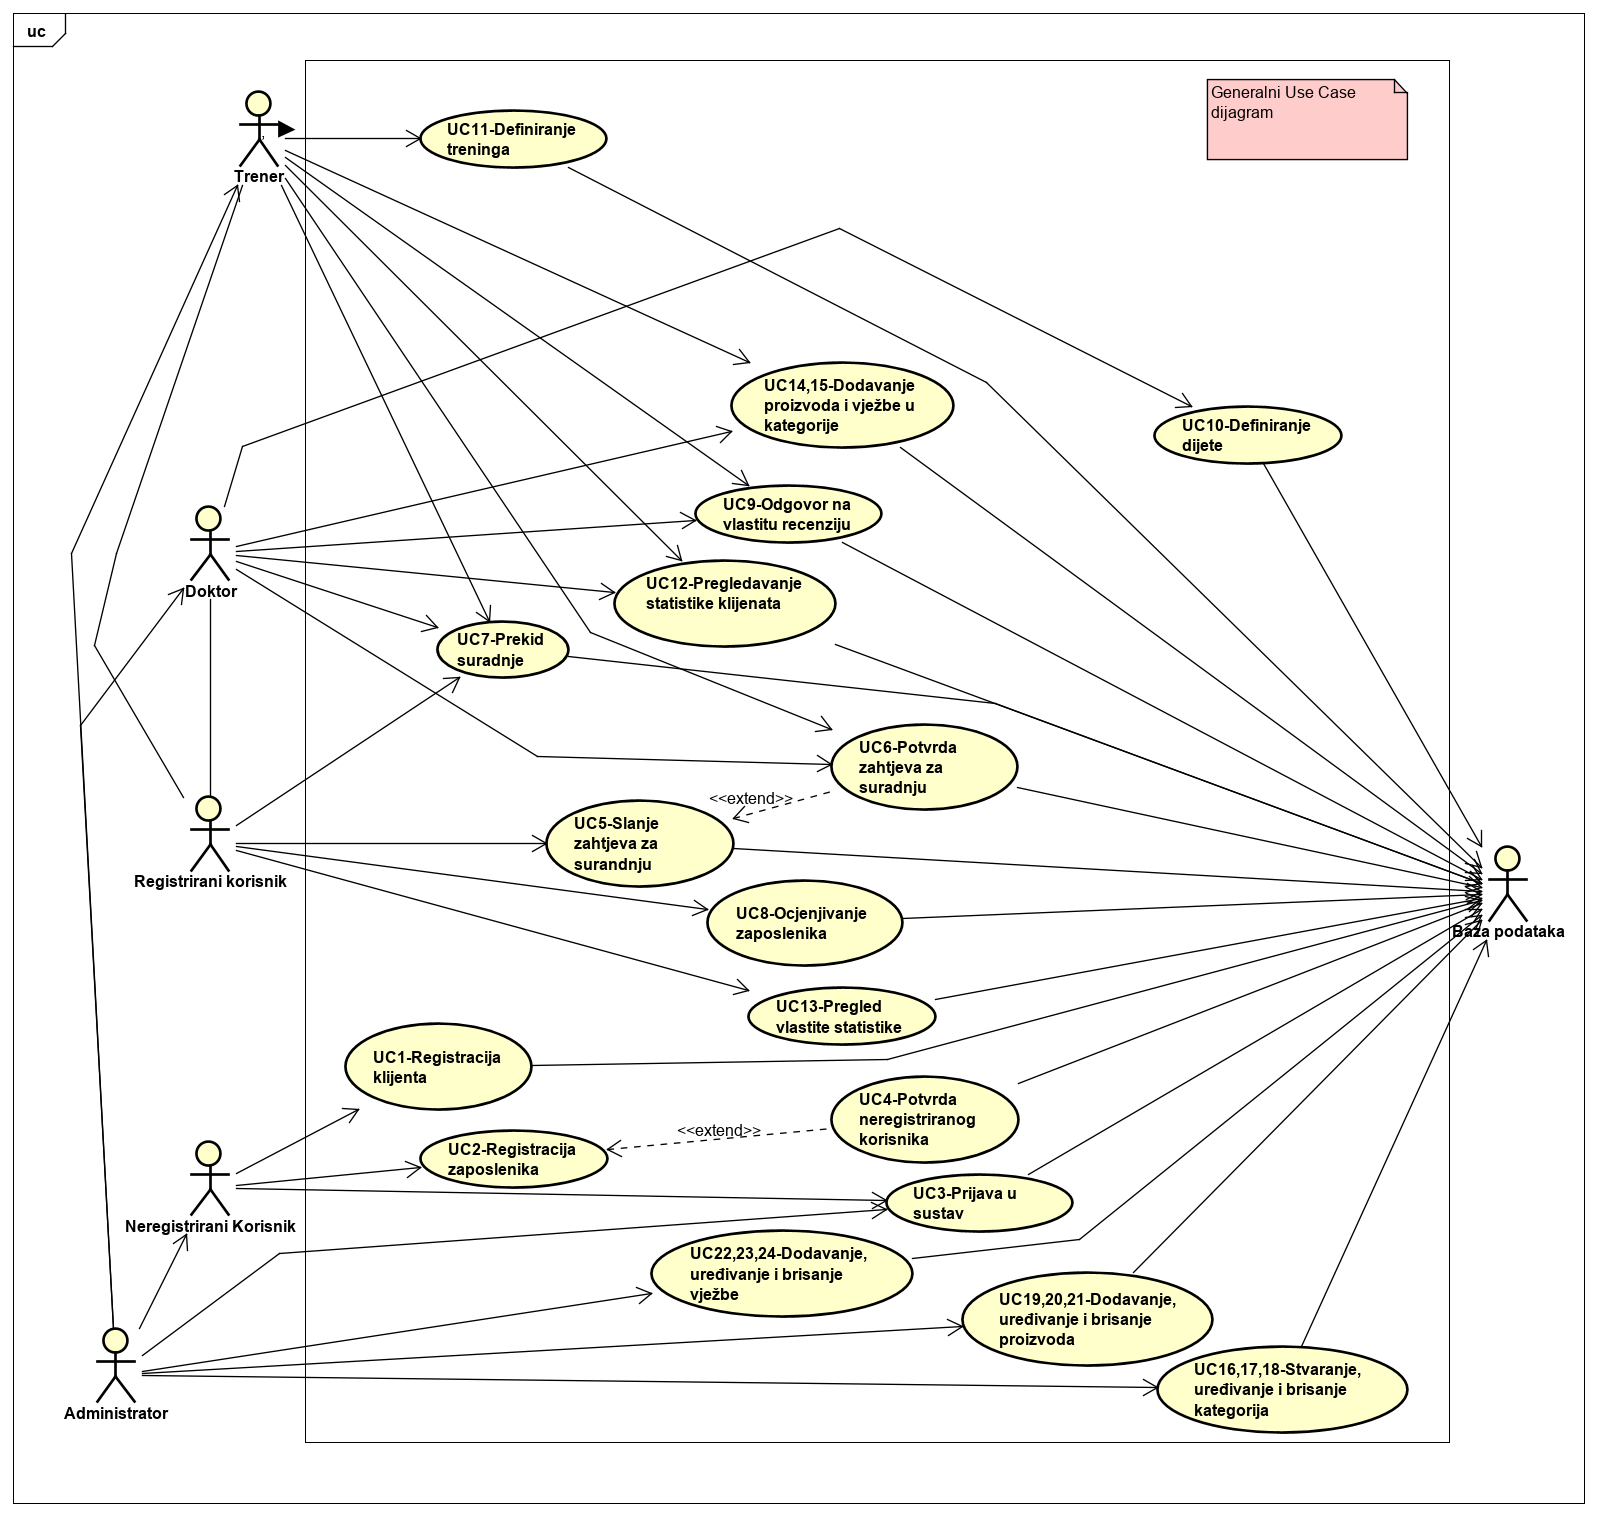
\includegraphics[scale=0.40]{dijagrami/UseCase/UseCase Diagram0.PNG}
						\centering
						\caption{Generalni dijagram obrasca uporabe}
						\label{fig:promjene}
					\end{figure}
				
					\begin{figure}[H]
						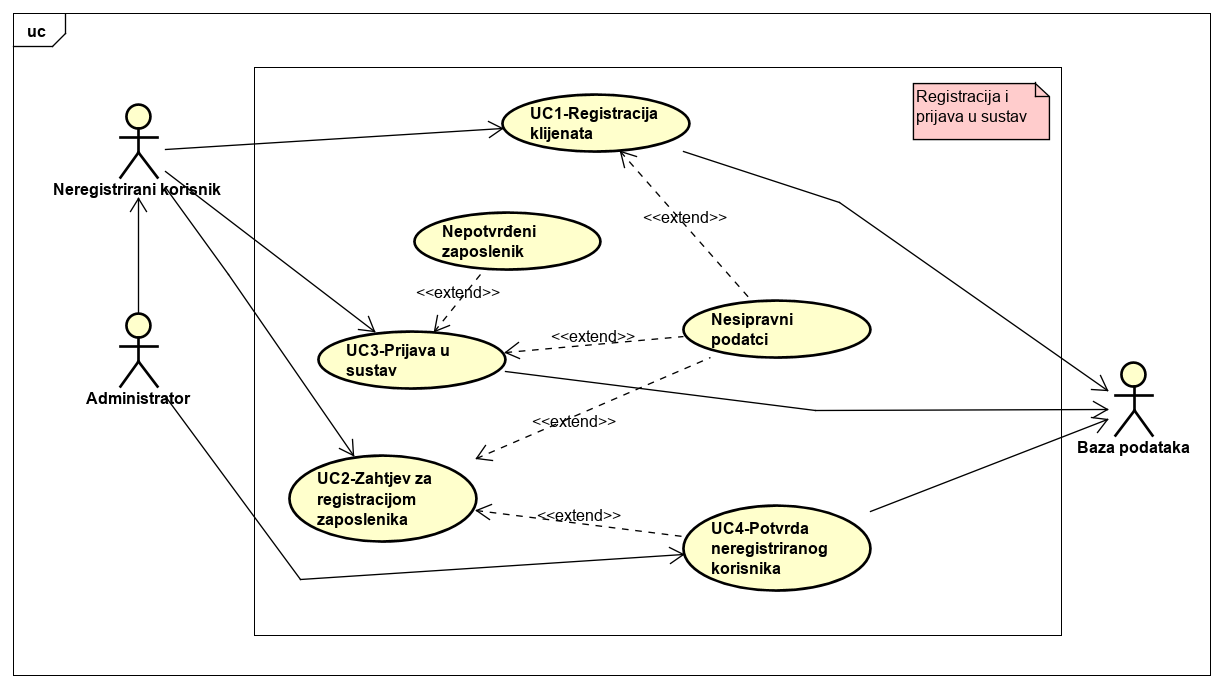
\includegraphics[scale=0.50]{dijagrami/UseCase/UseCase Diagram1.PNG}
						\centering
						\caption{Dijagram obrasca uporabe - registracija i prijava}
						\label{fig:promjene}
					\end{figure}
				
					\begin{figure}[H]
						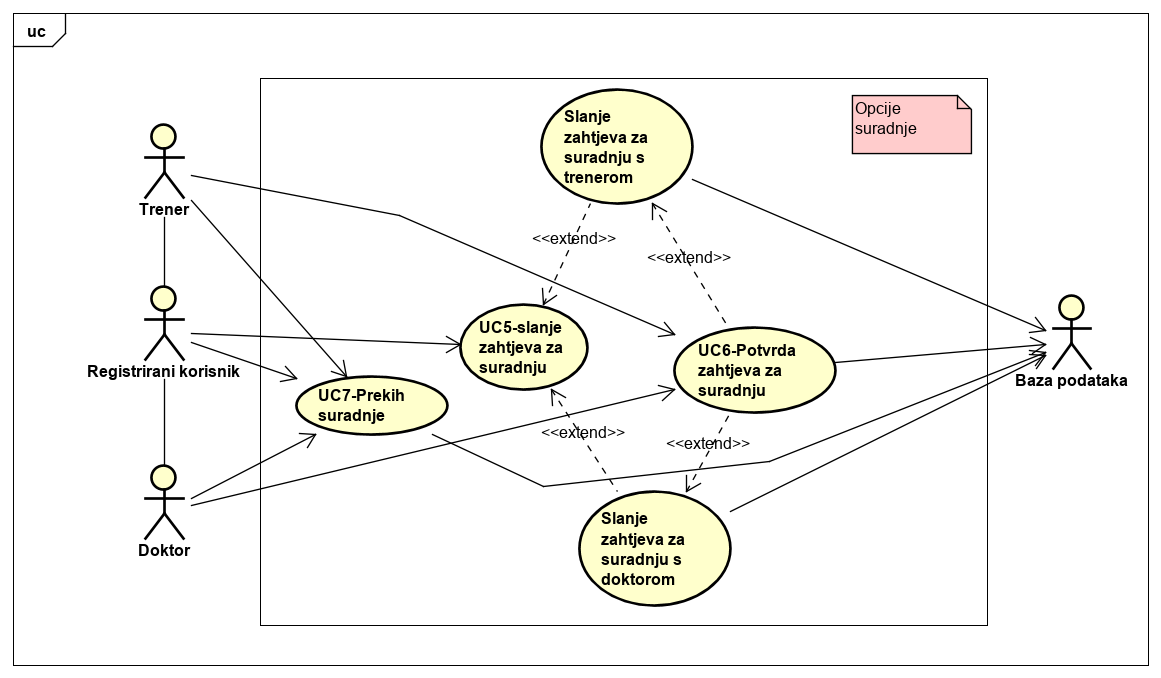
\includegraphics[scale=0.50]{dijagrami/UseCase/UseCase Diagram2.PNG}
						\centering
						\caption{Dijagram obrasca uporabe - opcije suradnje}
						\label{fig:promjene}
					\end{figure}
				
					\begin{figure}[H]
						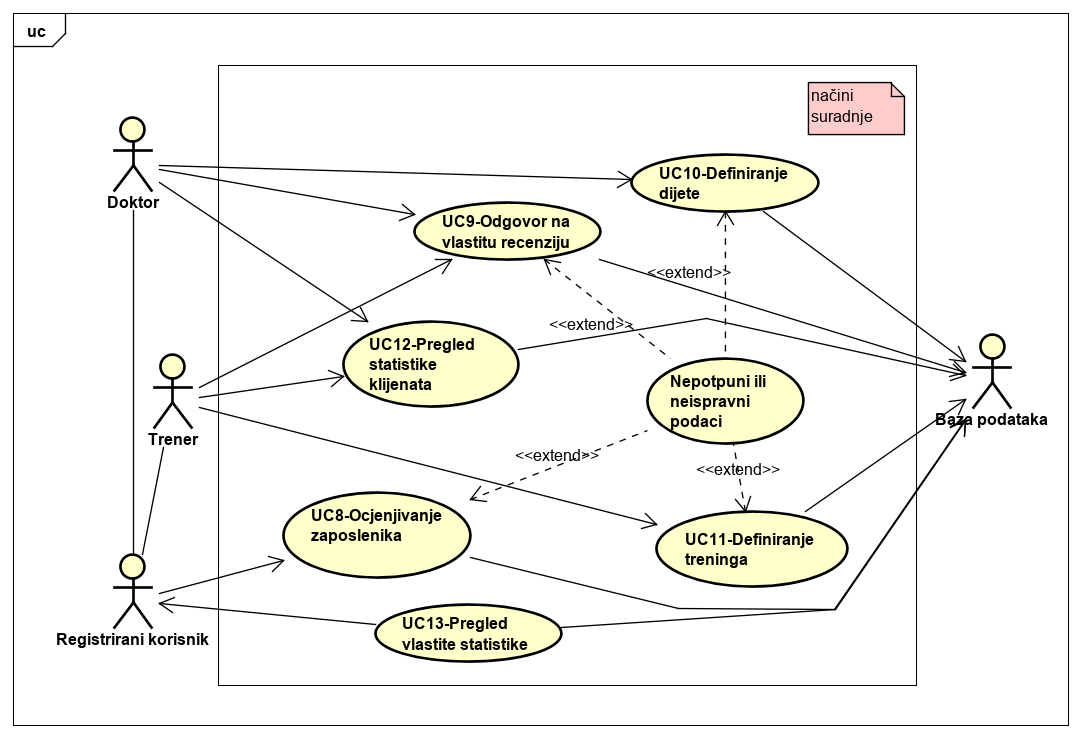
\includegraphics[scale=0.50]{dijagrami/UseCase/UseCase Diagram3.PNG}
						\centering
						\caption{Dijagram obrasca uporabe - načini suradnje}
						\label{fig:promjene}
					\end{figure}
				
					\begin{figure}[H]
						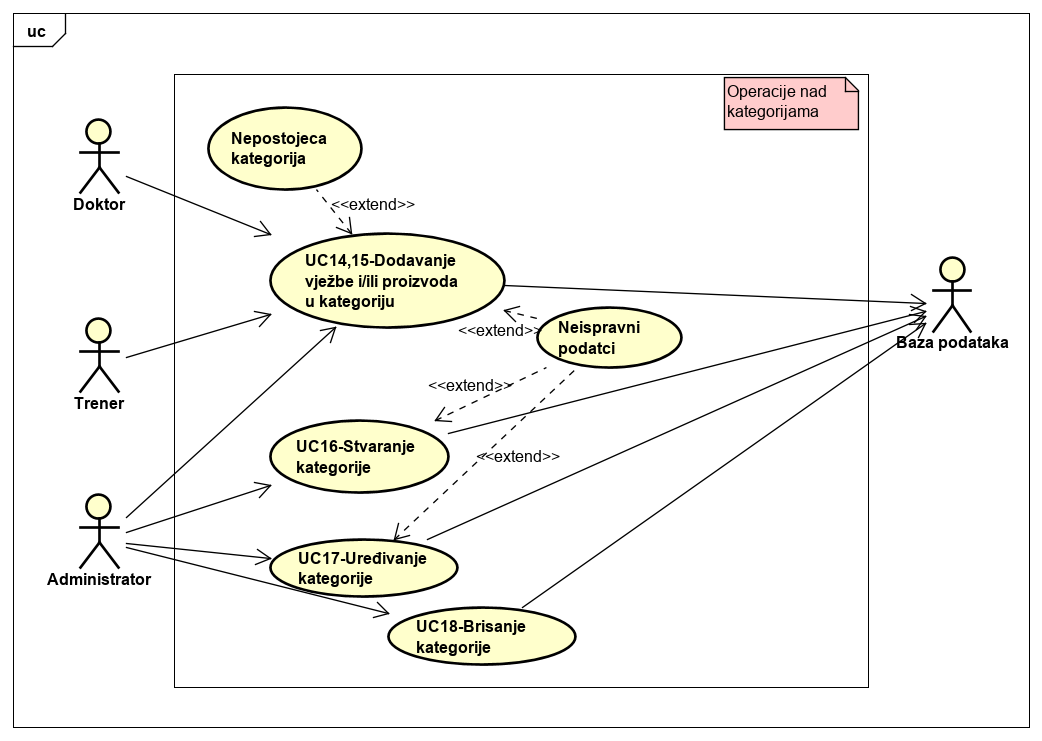
\includegraphics[scale=0.50]{dijagrami/UseCase/UseCase Diagram4.PNG}
						\centering
						\caption{Dijagram obrasca uporabe - operacije nad kategorijama}
						\label{fig:promjene}
					\end{figure}
				
					\begin{figure}[H]
						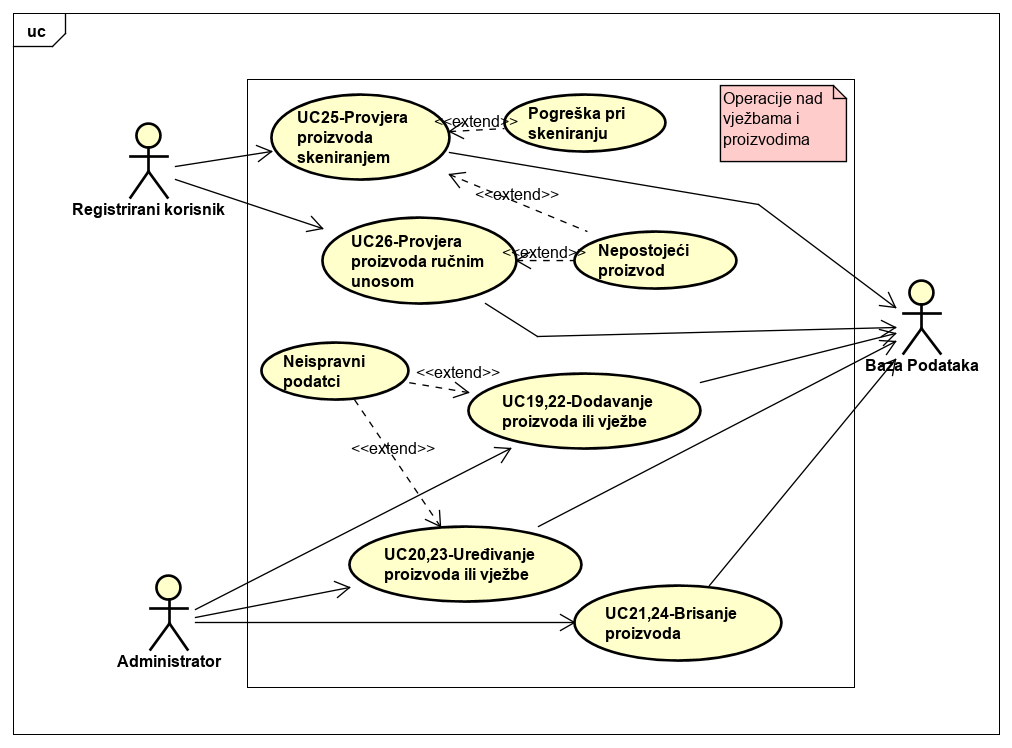
\includegraphics[scale=0.50]{dijagrami/UseCase/UseCase Diagram5.PNG}
						\centering
						\caption{Dijagram obrasca uporabe - operacije nad vježbama i proizvoidma}
						\label{fig:promjene}
					\end{figure}
				
			\subsection{Sekvencijski dijagrami}
				
				\textbf{\textit{dio 1. revizije}}\\
				
				\textit{Nacrtati sekvencijske dijagrame koji modeliraju najvažnije dijelove sustava (max. 4 dijagrama). Ukoliko postoji nedoumica oko odabira, razjasniti s asistentom. Uz svaki dijagram napisati detaljni opis dijagrama.}
				\eject
	
		\section{Ostali zahtjevi}
			 
			 \begin{packed_item}
			 	
			 	\item Pristup aplikaciji mora biti omogućen iz javne mreže pomoću HTTPS-a.
			 	\item Veza s bazom podataka mora biti sigurna i kvalitetna. Također veza mora biti brza.
			 	\item Nadogradnja sustava mora biti moguća.
			 	\item Sustav mora biti jednostavan za korištenje.
			 	\item Kratke upute o korištenju moraju biti omogućene.
			 	\item Obavijestiti korisnika o neispravnom korištenju sučelja.
			 	\item Neispravno korištenje sučelja ne smije narušiti rad aplikacije.
			 	\item Sustav mora biti implementiran kao web-aplikacija pomoću objektno orijentiranih jezika.
			 	\item Sustav mora podržavati rad više korisnika u istome trenutku.
			 	\item Aplikacija mora podržavati hrvatsku abecedu.
			 	
			 \end{packed_item}
			 
			 
	